\chapter{Návrh riešenia}\label{ch:návrh}

\section{Demonštrácia riešenia}\label{sec:demonstracia-riesenia}

Prvým krokom pri návrhu riešenia, bolo z pohľadu informačnej bezpečnosti presne zadefinovať a rozanalyzovať hlavné prípady
použitia.
Medzi hlavné prípady použitia, ktoré boli zadefinované s cieľom formovania myšlienky boli napríklad: Konfigurovateľná správa
vnútorno-firemnej bezpečnostnej politiky v nami navrhnutej webovej aplikácii, prísne zadefinovaná hierarchia a vzťah medzi objektami,
riadenie celého procesu nasadenia, alternatívne možnosti prístupov s bezpečným dohľadom nad všetkými operáciami a komunikačnými správami.
Medzi najhlavnejšie kritéria, ktorými bol riadený celý proces návrhu boli bezpečnosť a modularita riešenia.
Preto bolo zadefinovaných päť majoritných entít: webové api, ssh proxy server, api klient, používateľ a koncové zariadenie.
Tieto vymenované entity medzi sebou komunikujú a interagujú v presne zadefinovanej a zabezpečenej schéme, ktorú môžme vidieť
v nasledujúcom grafickom náhľade riešenia~\ref{fig:obr_8}.

\begin{figure}[H]
\begin{center}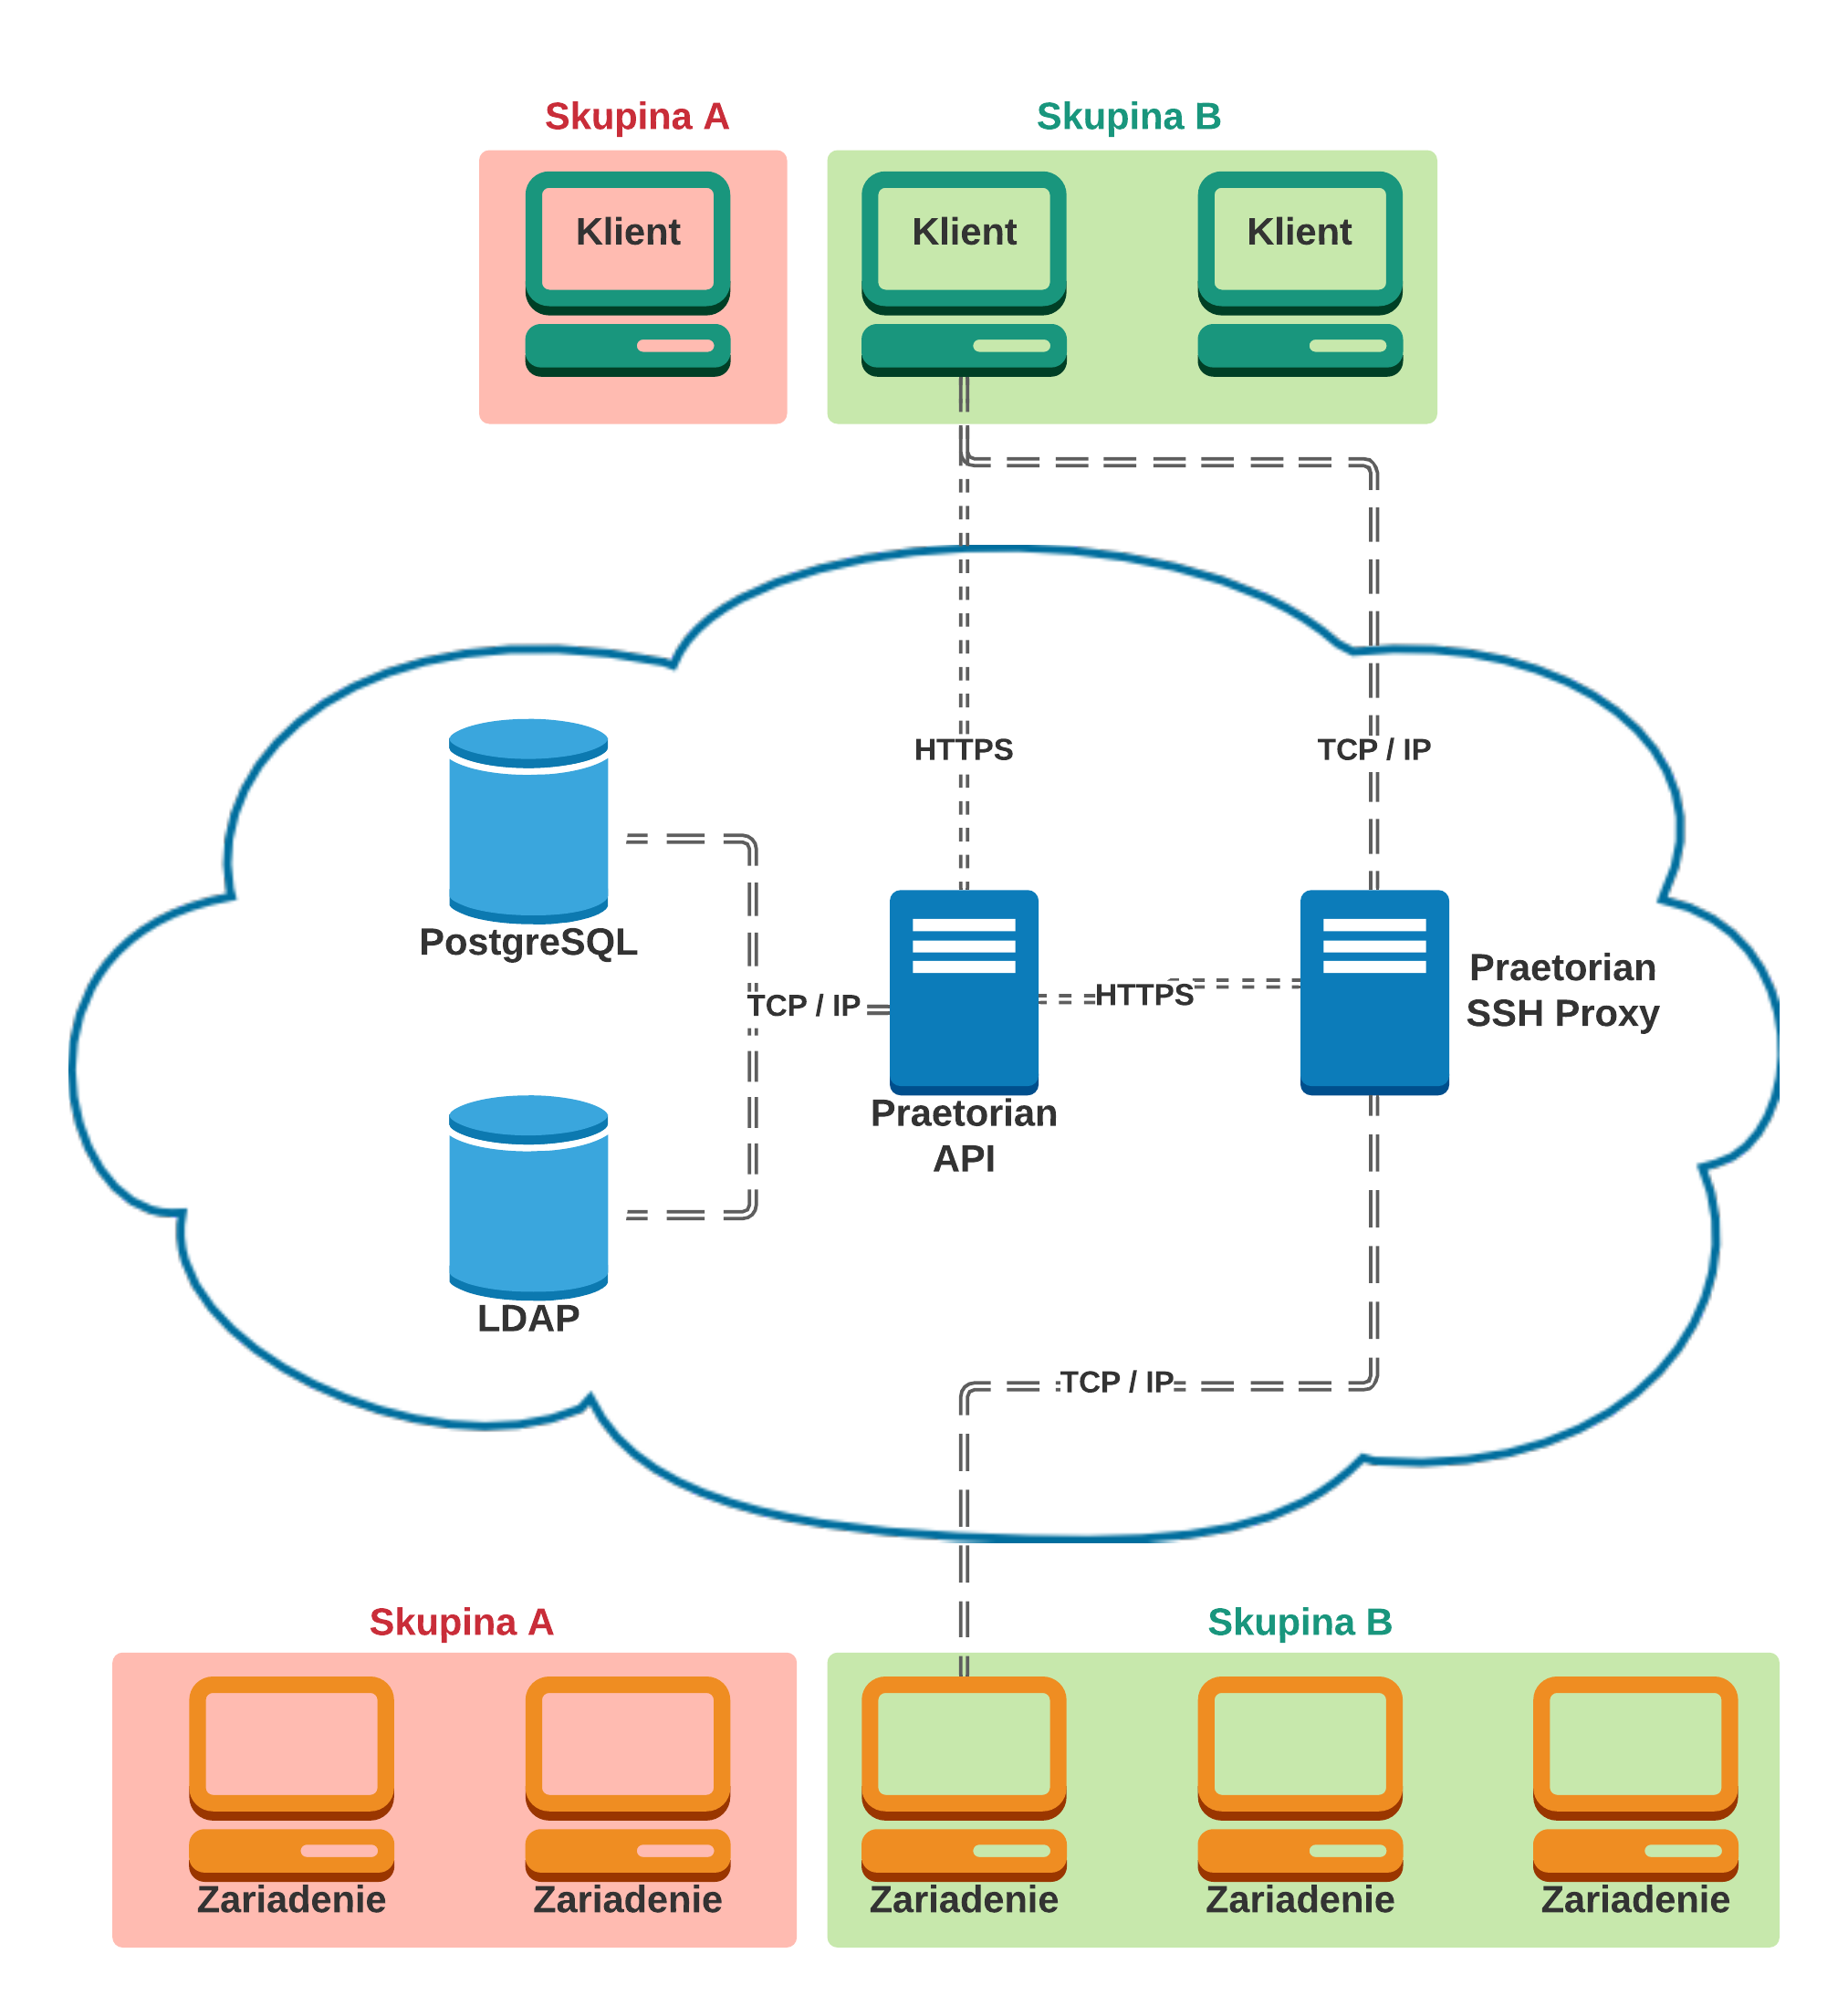
\includegraphics[width=\textwidth,height=12cm,keepaspectratio=true]{assets/demonstracia_riesenia.png}\end{center}
\caption[Náhľad riešenia]{Náhľad riešenia}\label{fig:obr_8}
\end{figure}

Z náhľadu je možné vidieť klientov, ktorí predstavujú bežných používateľov navrhovaného systému.
Môžu sa medzi sebou líšiť svojou rolou v systéme, projektom, ktorý im je pridelený, zoznamom práv a zariadení s ktorými
daný používatelia majú dovolené pracovať, alebo dokonca typom siete, z ktorej sa na daný systém pripájajú.
Všetky tieto aspekty sú systémom sledované a vyhodnocované z pohľadu informačnej bezpečnosti.

Používateľ môže komunikovať s dvoma typmi komponentov.
Prvým je webová aplikácia, ktorá zastrešuje celý systémový manažment, spravuje operácie nad firemnými údajmi a kontroluje
ich správnosť.
Webová aplikácia môže komunikovať s rôznymi typmi dátových úložisk, pričom autentifikácia pokrýva možnosť prihlásenia cez
vnútornú databázu systému, alebo cez protokol ľahkého prístupu k adresáru (Lightweight Directory Access Protocol - LDAP).
To umožňuje jednoduchú správu a migráciu firemných zamestnancov v systéme.
Druhým komponentom je ssh proxy server, ktorého hlavnou úlohou je zabezpečenie komunikácie medzi klientom a vzdialeným
zariadením bez toho, aby obe komunikujúce strany o sebe vedeli.
Komponent funguje, ako tretia strana anonymizujúca a kontrolujúca celý komunikačný proces medzi dvoma bodmi, s možnosťou
auditovateľnosti posielaných správ, či ich filtrovania podľa presne nastavených noriem (ako napríklad whitelist, alebo blacklist).
Taktiež významnou úlohou ssh proxy servera je možnosť bezpečnej komunikácie s webovým api, pričom komunikácia predovšetkým
slúži na kontrolu a validáciu procesu autentifikácie, autorizácie, alebo správu privilegovaného prístupu k potrebným citlivým
údajom za pomoci vlastného špecializovaného api kľúča.

Práve tento nami navrhnutý ssh proxy server umožňuje kľúčovú funkcionalitu, ktorou sa naša práca výrazne odlišuje oproti
existujúcim riešeniam.
Tou je automatizované nasadenie produktu a komunikácia s koncovými zariadeniami bez potreby používateľa akýmkoľvek spôsobom pristúpiť,
alebo interagovať s citlivými a prístupovými údajmi.
Zahájenie tohto druhu operácie si vyžaduje adresu, port ssh proxy servera a osobné prístupové údaje používateľa do systému.
Prístupovými údajmi je možné na strane api servera skontrolovať používateľovu identitu a oprávnenia týkajúce sa miery manipulácie
medzi daným projektom, koncovým zariadením, sieťou, z ktorej sa daná operácia uskutočňuje a zariadením, z ktorého sa akcia vykonáva.
Citlivé údaje sú v databáze systému uložené spôsobom názov-hodnota, pričom k hodnotám má podľa miery dôveryhodnosti prístup buď
iba ssh proxy server, alebo aj samotný používateľ.
Validácia prístupu k týmto údajom je umožnená za pomoci rozdielnych api kľúčov, ktoré sú vyhodnocované api serverom.
Zatiaľ, čo hodnoty citlivých údajov podliehajú validácii, názvy sú používateľovi známe aj pri dôverných (skrytých) informáciach.
Jednotlivé príkazy, ktoré majú obsahovať hodnoty citlivých údajov používateľ nahradí názvom.
Po odoslaní príkazu je možné zo strany ssh proxy servera vykonať požiadavku na api server pod privilegovaným api kľúčom.
Týmto spôsobom si vie názvy dôverných informácií nahradiť hodnotami, a následne príkaz odoslať na anonymizované koncové zariadenie.
Keďže má ssh proxy server prístup k vzdialeným zariadeniam aj prístupovým údajom na rôzne technológie (dátové úložisko, environment premenné, ldap),
bezpečnosť celého riešenia môže byť zvýšená o dodatočnú funkcionalitu automatizovaného dynamického menenia prístupových údajov
podľa nastaveného časového intervalu.

\section{Diagram komponentov}\label{sec:diagram-komponentov}

S prihliadnutím na veľmi vysokú modularitu a rozšíriteľnosť riešenia bol systém a jeho dôležité komponenty dopodrobna rozanalyzovaný.
Médiom znázorňujúcim závislosti medzi softvérovými komponentami, ako napríklad triedy a ich navrhovaný vzťah medzi
nimi sa nazýva diagram komponentov.
Keďže sa jedná o veľmi komplexné riešenie, prihliadali sme z dôvodu prehľadnosti na abstrahovanie problému v čo najvyššej miere.
Výsledný diagram komponentov~\ref{fig:obr_9}~zobrazený nižšie, znázorňuje vzťahy tých komponentov, ktoré sú nevyhnutné pre
získanie vzdialeného prístupu ku koncovému zariadeniu.

\begin{figure}[H]
\begin{center}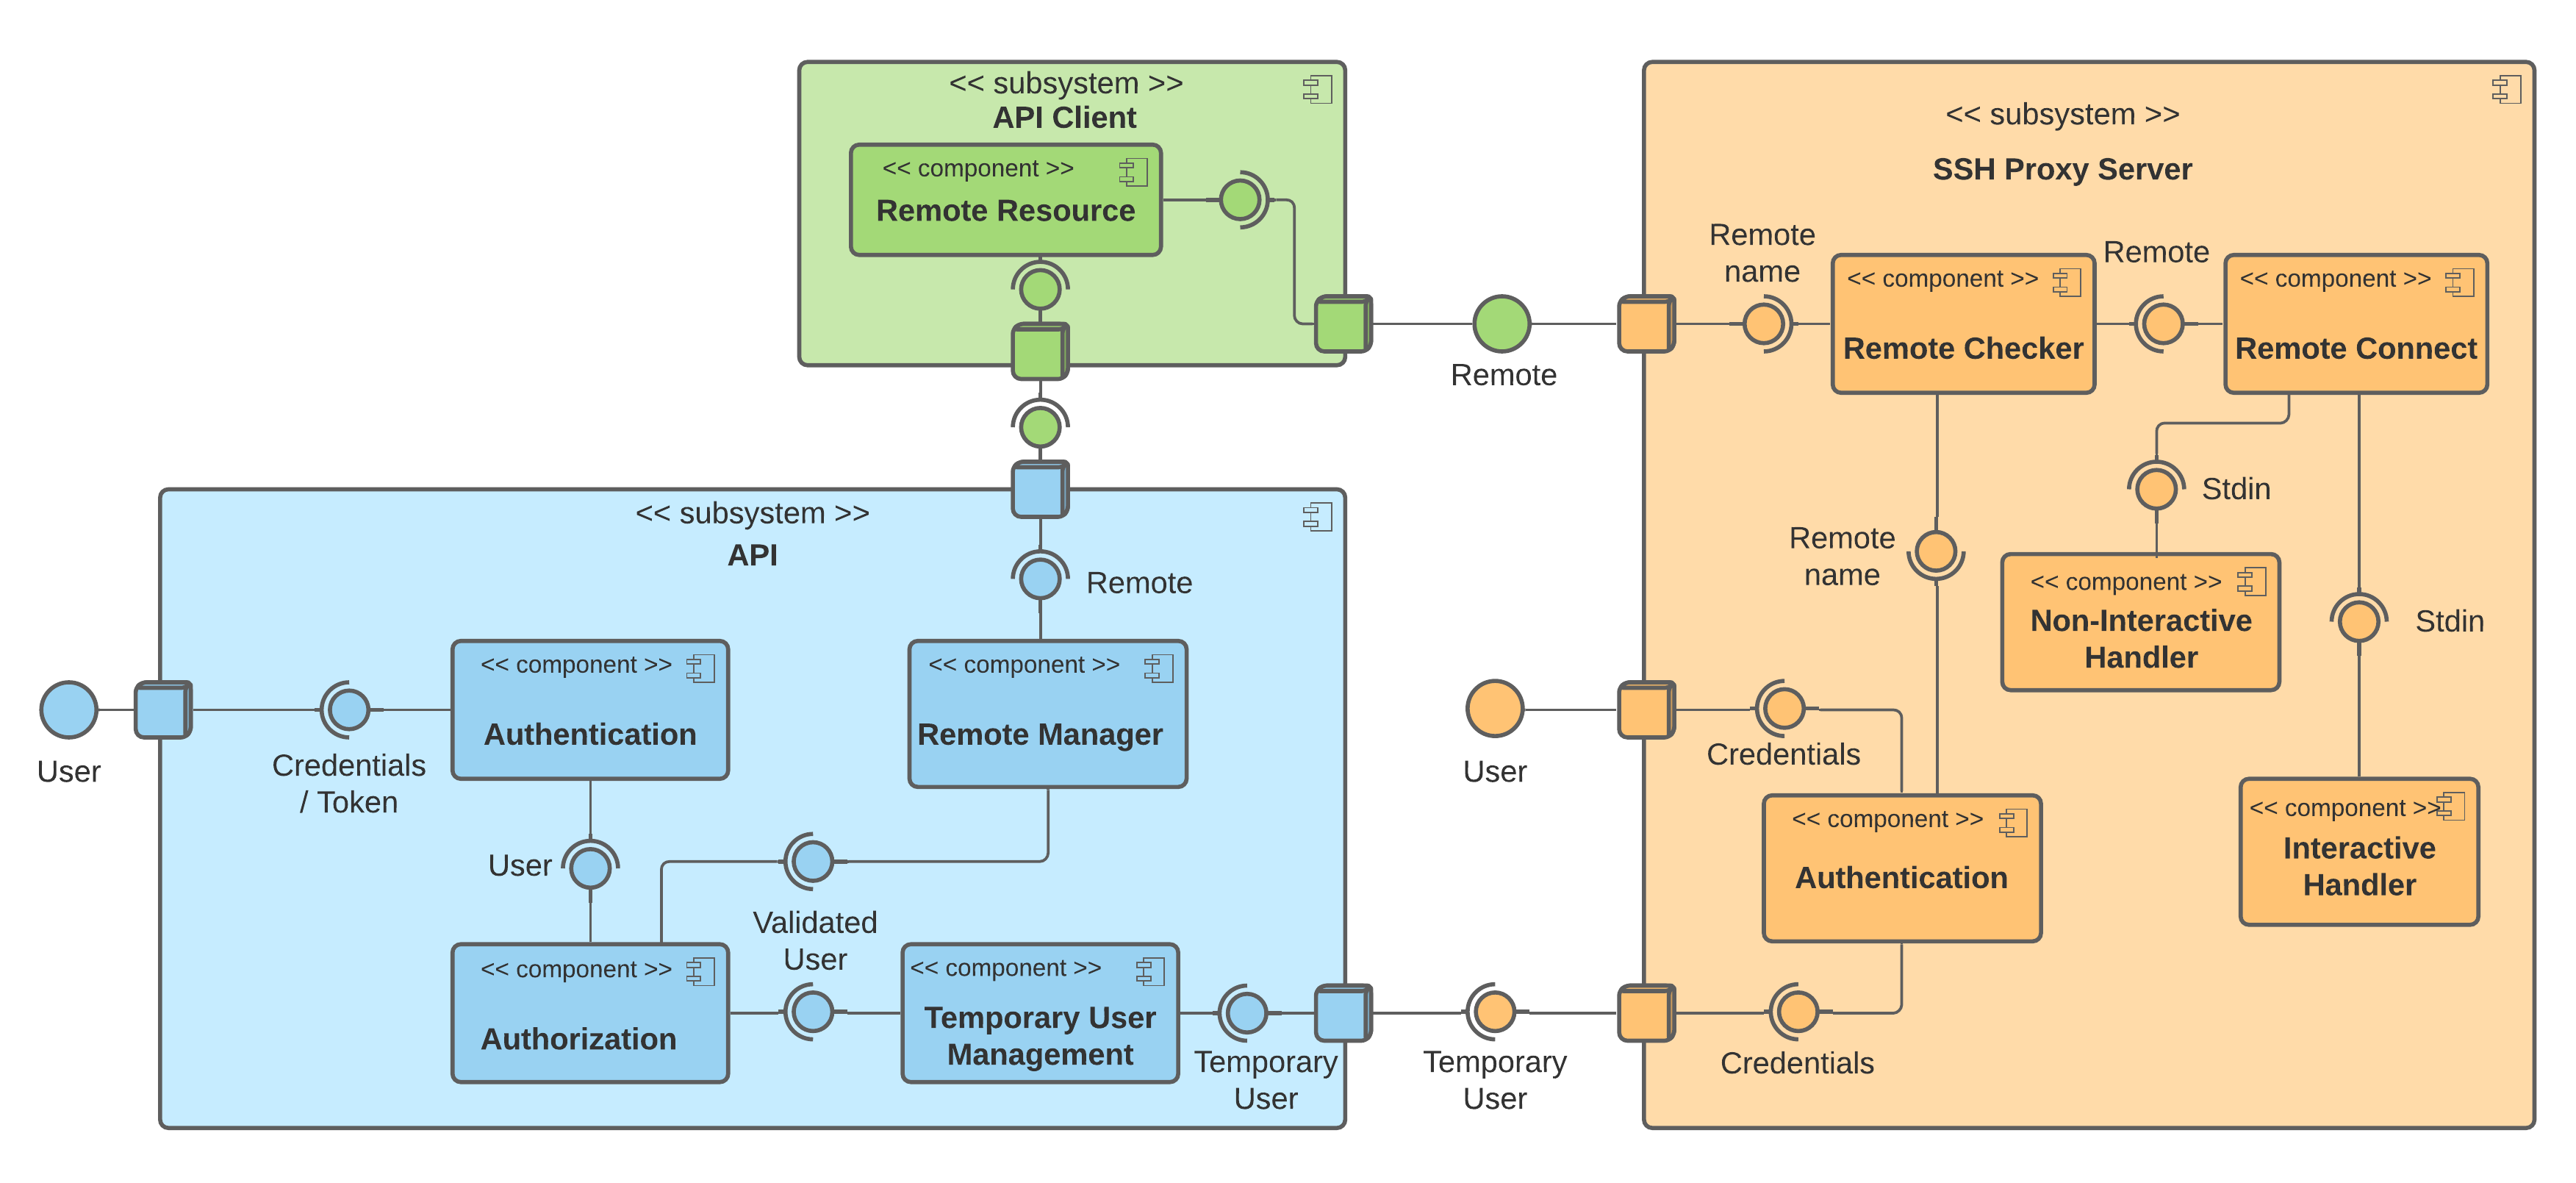
\includegraphics[width=\textwidth,height=8cm,keepaspectratio=true]{assets/diagram_komponentov.png}\end{center}
\caption[Diagram komponentov]{Diagram komponentov}\label{fig:obr_9}
\end{figure}

Ako je v diagrame znázornené, celý navrhovaný systém sa skladá z troch hlavných komponentov: webové api, api klient a ssh proxy server.
Komunikácia medzi webovým api a ssh proxy serverom prebieha cez api klienta, ktorý zvyšuje modularitu, bezpečnosť, udržiavateľnosť a
auditovateľnosť celého riešenia.
V systéme figurujú dva hlavné typy používateľov, a to štandardný permanentný používateľ, ktorý sa môže prihlásiť do webovej
aplikácie a súčasne, ak je mu to oprávnené, môže komunikovať so vzdialeným zariadením cez ssh proxy server v interaktívnej
relácii ssh (interactive ssh session).
Druhým typom používateľa je dočasný, ktorého životnosť po vytvorení vo webovej aplikácii trvá iba obmedzený čas, alebo jeho
životnosť je ukončená súčasne s dokončením úlohy, pre ktorú bol vytvorený.
Dočasného používateľa je možné vytvoriť iba permanentným používateľom s prislúchajúcim oprávnením, pričom dočasný
používateľ je vytváraný s jediným cieľom, a tým je pripojenie sa na konkrétne vzdialené zariadenie.
Preto po tvorcovi „zdedí“ zvolený projekt a prístup ku konkrétnemu vzdialenému zariadeniu.
Tvorcovi následne príde notifikácia vo forme emailu o prístupových údajoch dočasného používateľa, pod ktorým je môže vykonať príkazy
v neinteraktívnej relácii ssh (non-interactive ssh session) cez ssh proxy server na koncové zariadenie.

\section{Sekvenčné diagramy}\label{sec:sekvencne-diagramy}

Keďže sa naše riešenie vo veľkej miere zaoberá vzájomnou komunikáciou medzi jednotlivými komponentami celého systému, je
veľmi dôležité pri návrhu zachytiť procesy, ktoré sa vykonávajú sekvenčne pri komunikácii.
Väčšina týchto procesov figuruje vo forme správ, ktoré si jednotlivé komponenty vymieňajú, a preto bolo pri návrhu daných
častí systému použitie sekvenčných diagramov optimálnou voľbou.

\subsection{Autentifikácia}\label{subsec:sek-autentifikacia}

Prvý sekvenčný diagram~\ref{fig:obr_10}~znázorňuje autentifikáciu prístupu používateľa k navrhovanému ssh proxy serveru.
Z pohľadu servera sa jedná o autentifikáciu klienta, ktorý môže byť permanentného, aj dočasného typu a taktiež musí patriť
do daného bezpečnostného systému.
Pre pripojenie k ssh proxy serveru je taktiež potrebné zistiť k akému koncovému zariadeniu sa používateľ chce pripojiť a
voči tomuto zvolenému zariadeniu skontrolovať autorizáciu pripájaného klienta.

\begin{figure}[H]
\begin{center}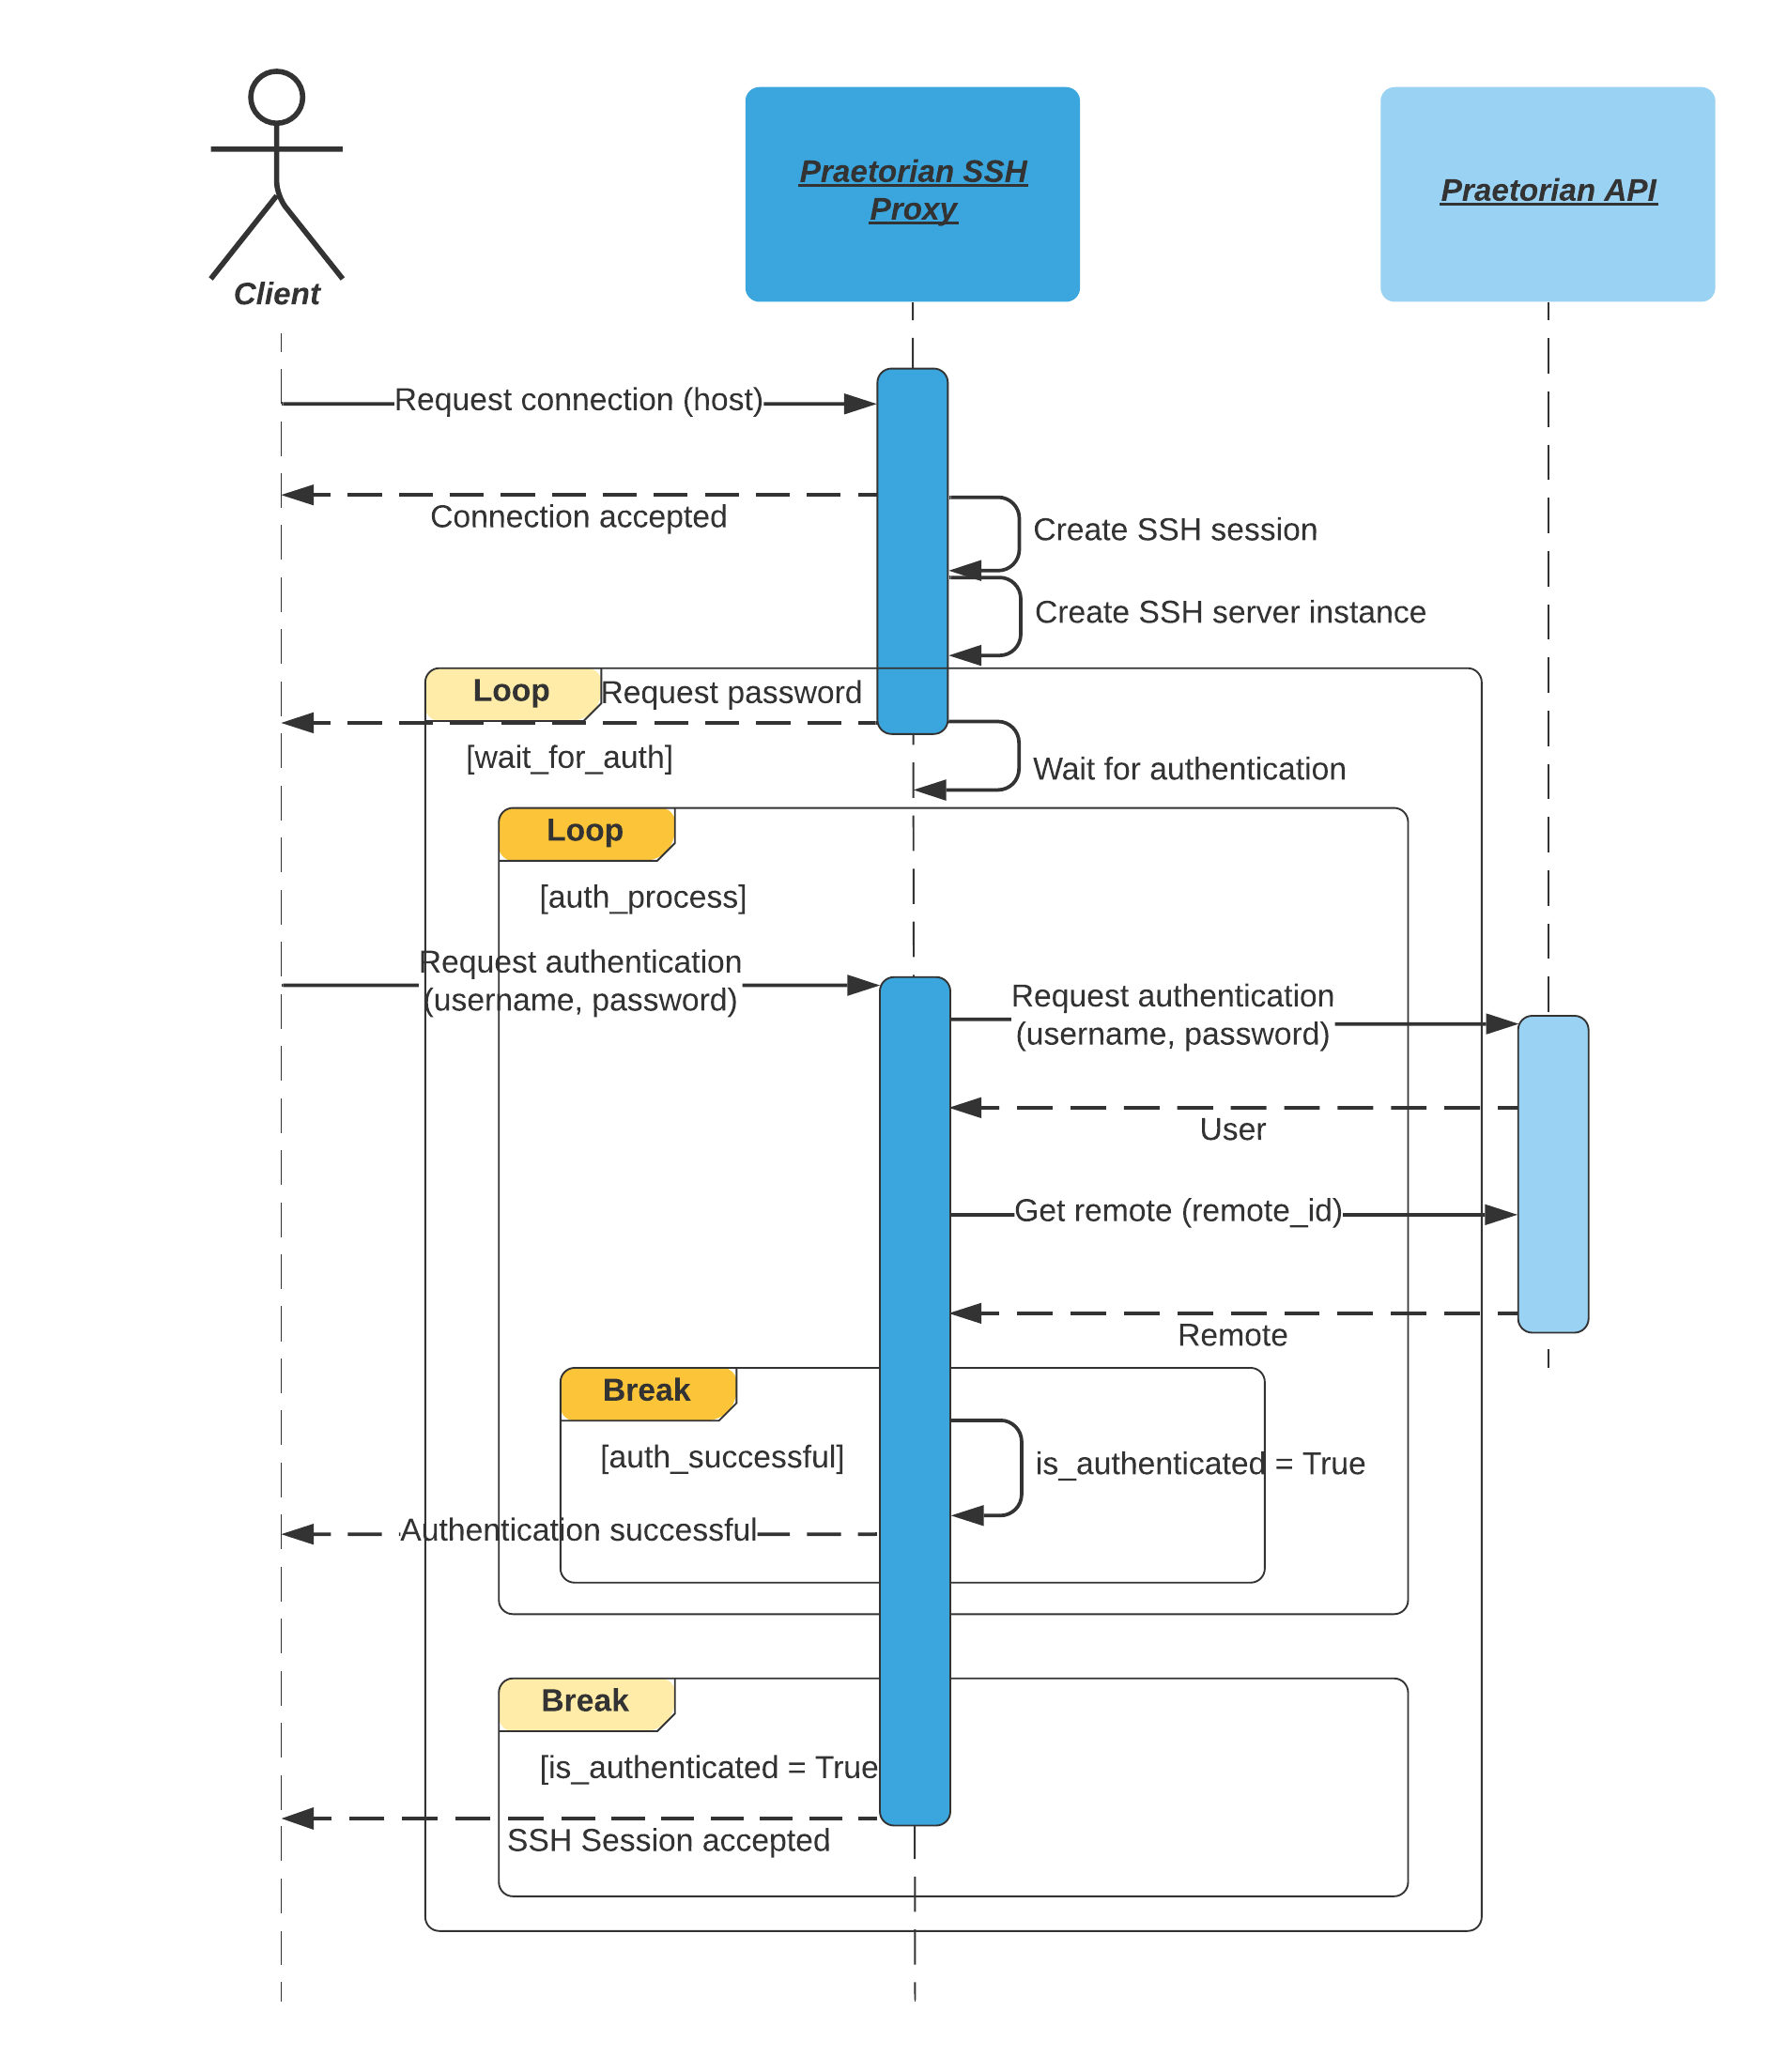
\includegraphics[width=\textwidth,height=15cm,keepaspectratio=true]{assets/sequence_diagram_auth.png}\end{center}
\caption[Autentifikácia]{Autentifikácia}\label{fig:obr_10}
\end{figure}

Ak sa chce klient pripojiť k ssh proxy serveru s úmyslom pripojenia sa na vzdialené zariadenie, musí si k serveru vyžiadať
prístup.
Po vyžiadaní prístupu server príjme daného klienta, umožnením komunikácie cez soket s cieľom otvorenia spojenia ssh.
Preto server vytvorí po pripojení klienta na daný soket novú ssh reláciu (ssh session) a následne vytvorí rozhranie ssh servera,
ktorého úlohou je spracovať vstup od klienta cez dané spojenie.
Proces vytvorenia rozhrania servera zároveň pošle klientovi požiadavku pre overenie pomocou hesla, pričom server čaká, dokiaľ
sa používateľ úspešne autentifikuje, alebo ukončí spojenie.
Po úspešnom zaslaní hesla, začína autentifikačný proces na strane servera, ktorý si overí správnosť pripájaného klienta vytvorením
novej inštancie api klienta s daným menom a heslom používateľa.
Ak sa api klient inštancia úspešne prihlási do webového api, ssh proxy server si cez api klienta vypýta dodatočné informácie o
používateľovi a koncové zariadenie.
Ak sú získané údaje z webového api validné, potom je autentifikácia úspešne ukončená a ssh relácia zo strany servera úspešne akceptovaná.

\subsection{Interaktívne prostredie}\label{subsec:interkativne-prostredie}

Druhý sekvenčný diagram~\ref{fig:obr_11}~zobrazuje proces vytvorenia a spracovania interaktívneho rozhrania ssh.
Tento typ pripojenia je umožnený iba permanentným používateľom systému a iba ku koncovým zariadeniam, ku ktorým majú daný
používatelia prístup.
Interaktívne prostredie ssh umožňuje simulovanie terminálu vzdialeného zariadenia, pričom pripojený používateľ môže v reálnom
čase posielať na dané zariadenie vstup vo forme príkazov, ktorých výstup im je následne zobrazovaný na výstupe.

\begin{figure}[H]
\begin{center}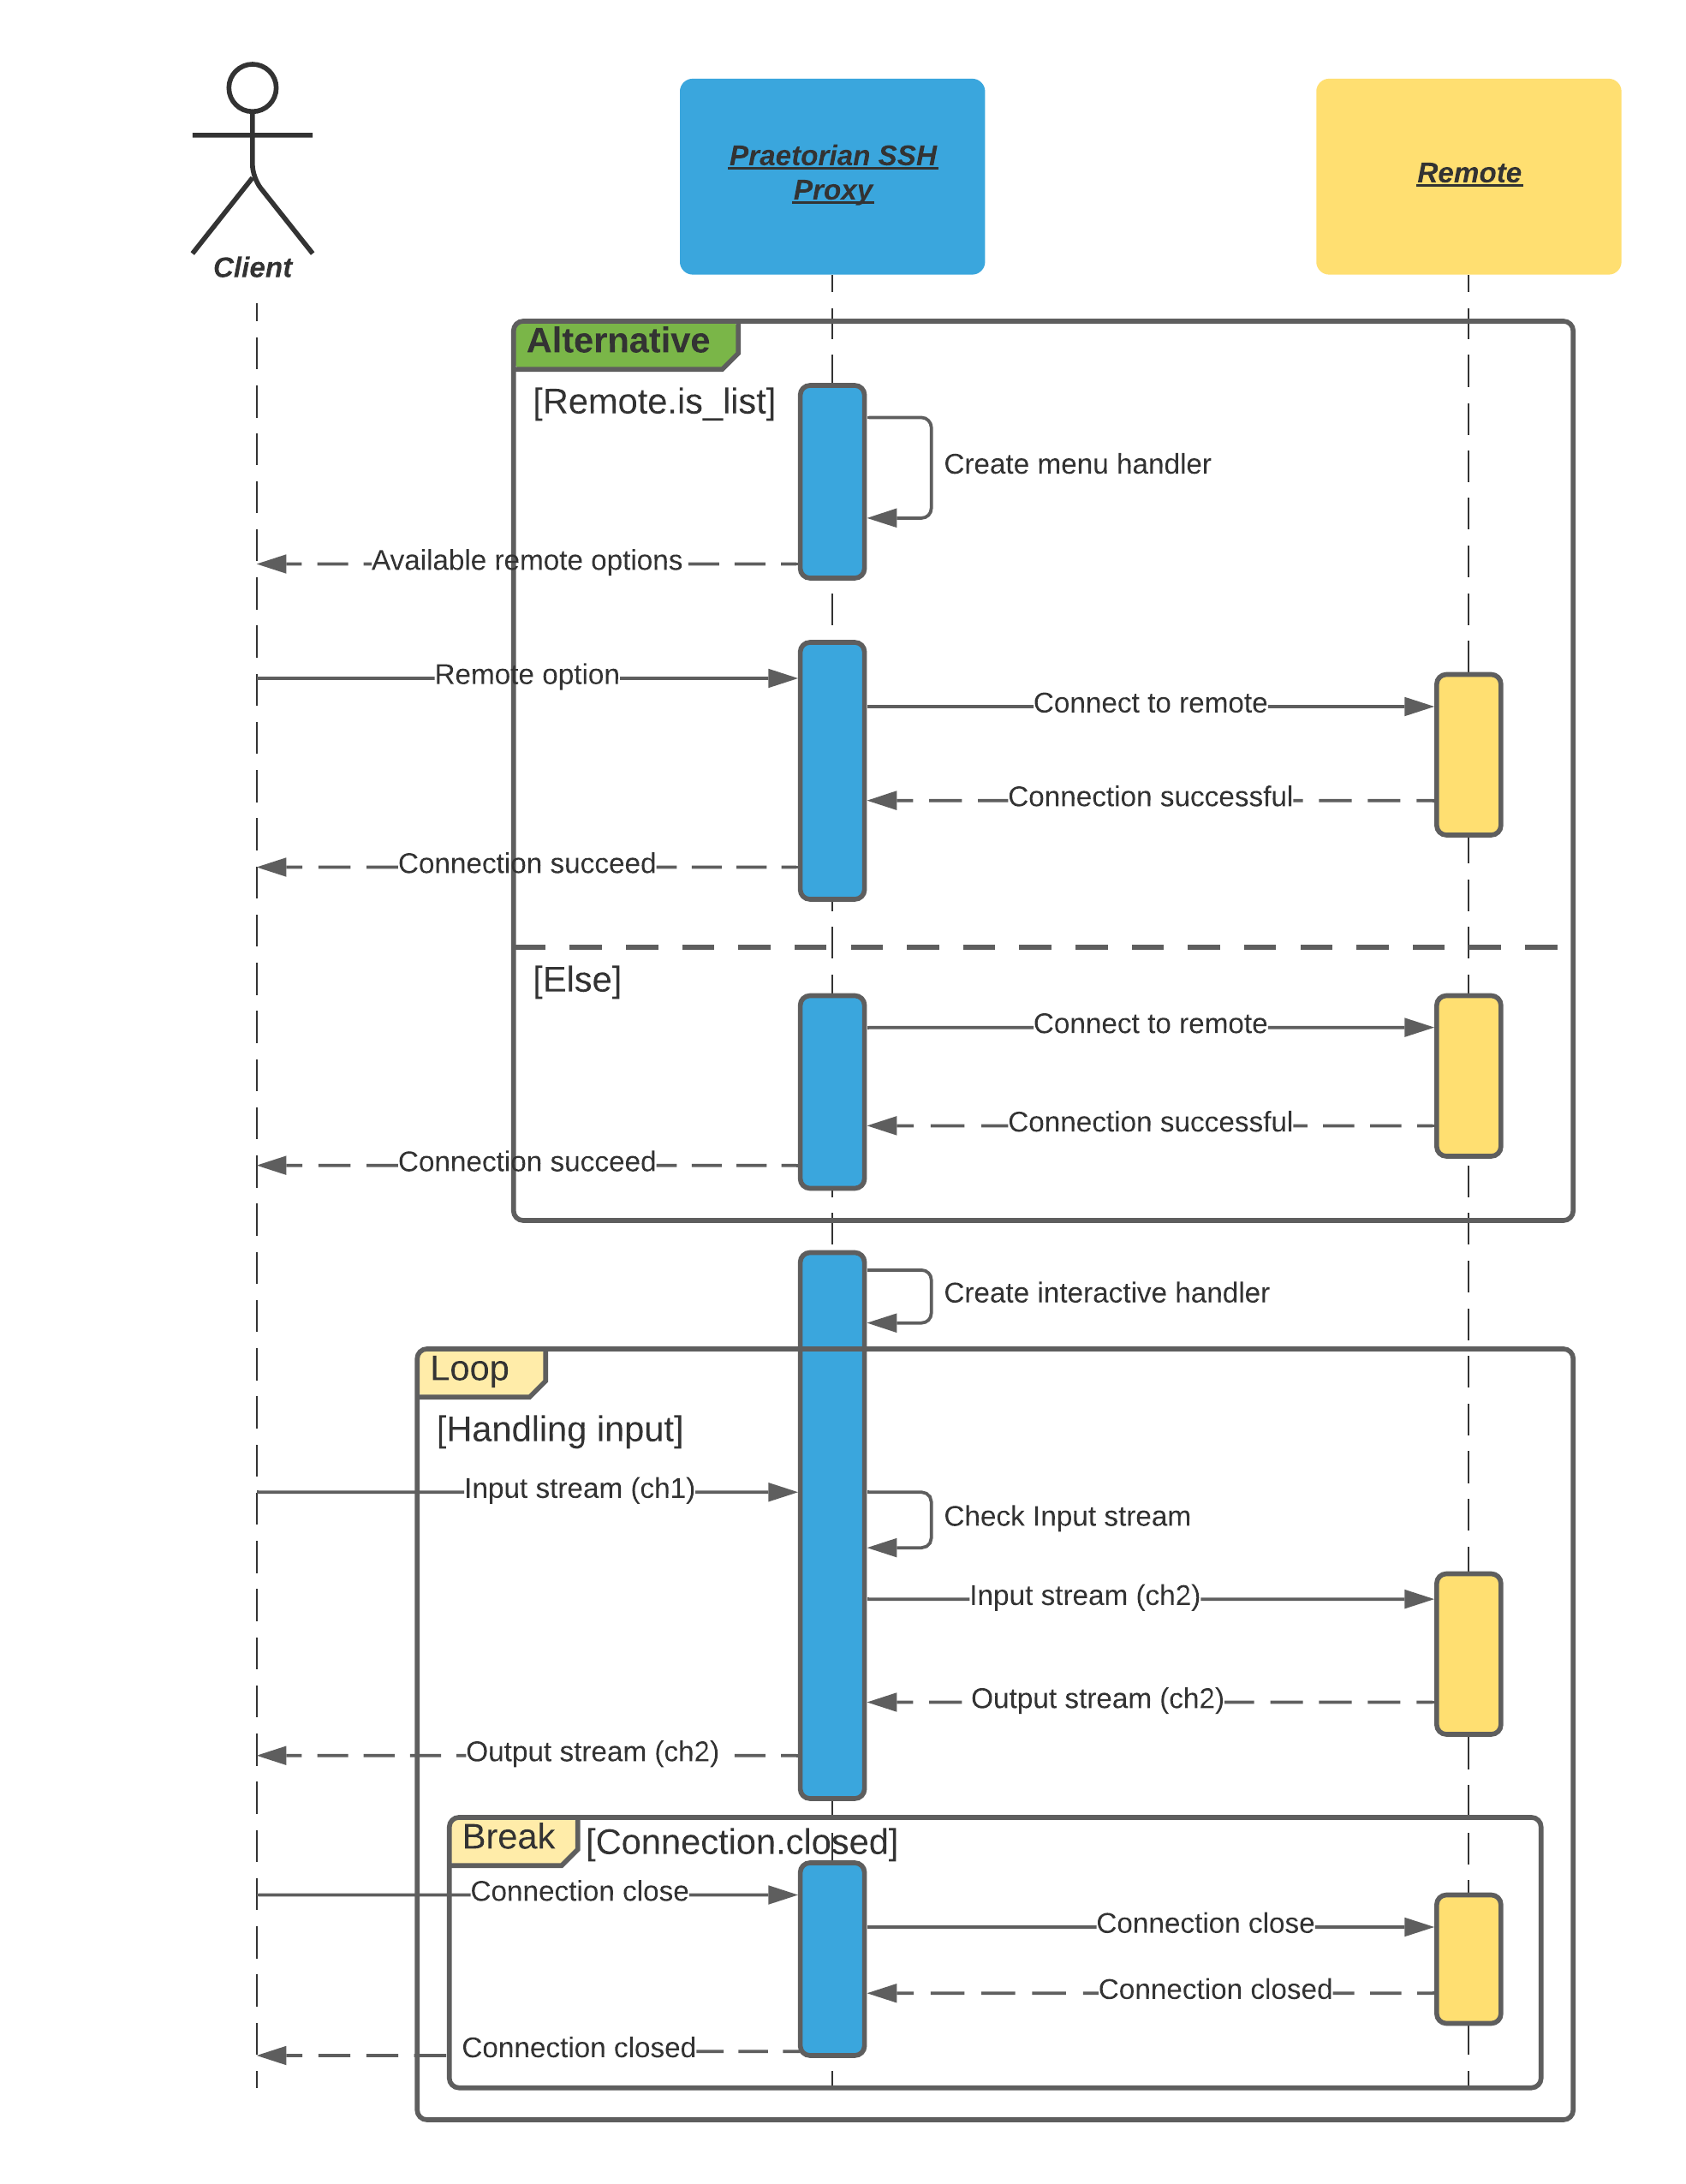
\includegraphics[width=\textwidth,height=15cm,keepaspectratio=true]{assets/sequence_diagram_interactive.png}\end{center}
\caption[Interaktívne prostredie]{Interaktívne prostredie}\label{fig:obr_11}
\end{figure}

Ak je úspešne autentifikovaný klient permanentným používateľom, má po pripojení k ssh proxy serveru dve možnosti.
Prvou je špecifikovanie vzdialeného zariadenia, ku ktorému sa chce klient pripojiť, alebo nešpecifikovať žiadne.
V prípade druhej z možností sa na strane ssh proxi servera vytvorí inštancia triedy „MenuHandler“, ktorá si z webového api
vyžiada zoznam dostupných koncových zariadení ku ktorým má daný používateľ právo.
Vytvorená inštancia následne vytvorí menu, z ktorého si používateľ môže vybrať práve jedno dané zariadenie.
Následne po vybraní zariadenia, proxy server požiada ssh server zariadenia o pripojenie s cieľom vzájomnej komunikácie.
Po úspešnom nadviazaní spojenia, proxy server vytvorí inštanciu triedy „InteractiveHandler“, ktorá zabezpečuje simuláciu
terminálu vzdialeného zariadenia.
Úlohou danej inštancie proxy servera je preposielanie vstupu z klienta na koncové zariadenie a spätné preposielanie výstupu
klientovi dovtedy, dokiaľ klient nepožiada o ukončenie spojenia.
Po vyžiadaní ukončenia spojenia zo strany klienta sa proxy server pokúsi uzavrieť spojenie so vzdialeným zariadením a nakoniec
uzavrie spojenie so samotným klientom.

\subsection{Neinteraktívne prostredie}\label{subsec:neinterkativne-prostredie}

Narozdiel od interaktívneho rozhrania, neinteraktívne rozhranie nesimuluje posielanie príkazov v reálnom čase, no slúži na
sekvenčné zaslanie príkazov pomocou skriptu, alebo súboru, pričom pri úspešnom dokončení sa spojenie ukončí a uzavrie.
K takémuto typu prostredia majú prístup iba dočasní používatelia, ktorý budú po vykonaní danej úlohy a po úspešnom ukončení spojenia
vymazaný.
Nasledujúci sekvenčný diagram~\ref{fig:obr_12}~graficky zobrazuje postup použitia daného prostredia, no taktiež pre úplnosť
celého postupu pri pripojení klienta na ssh proxy server obsahuje referencie na predchádzajúce dva sekvenčné diagramy.

\begin{figure}[H]
\begin{center}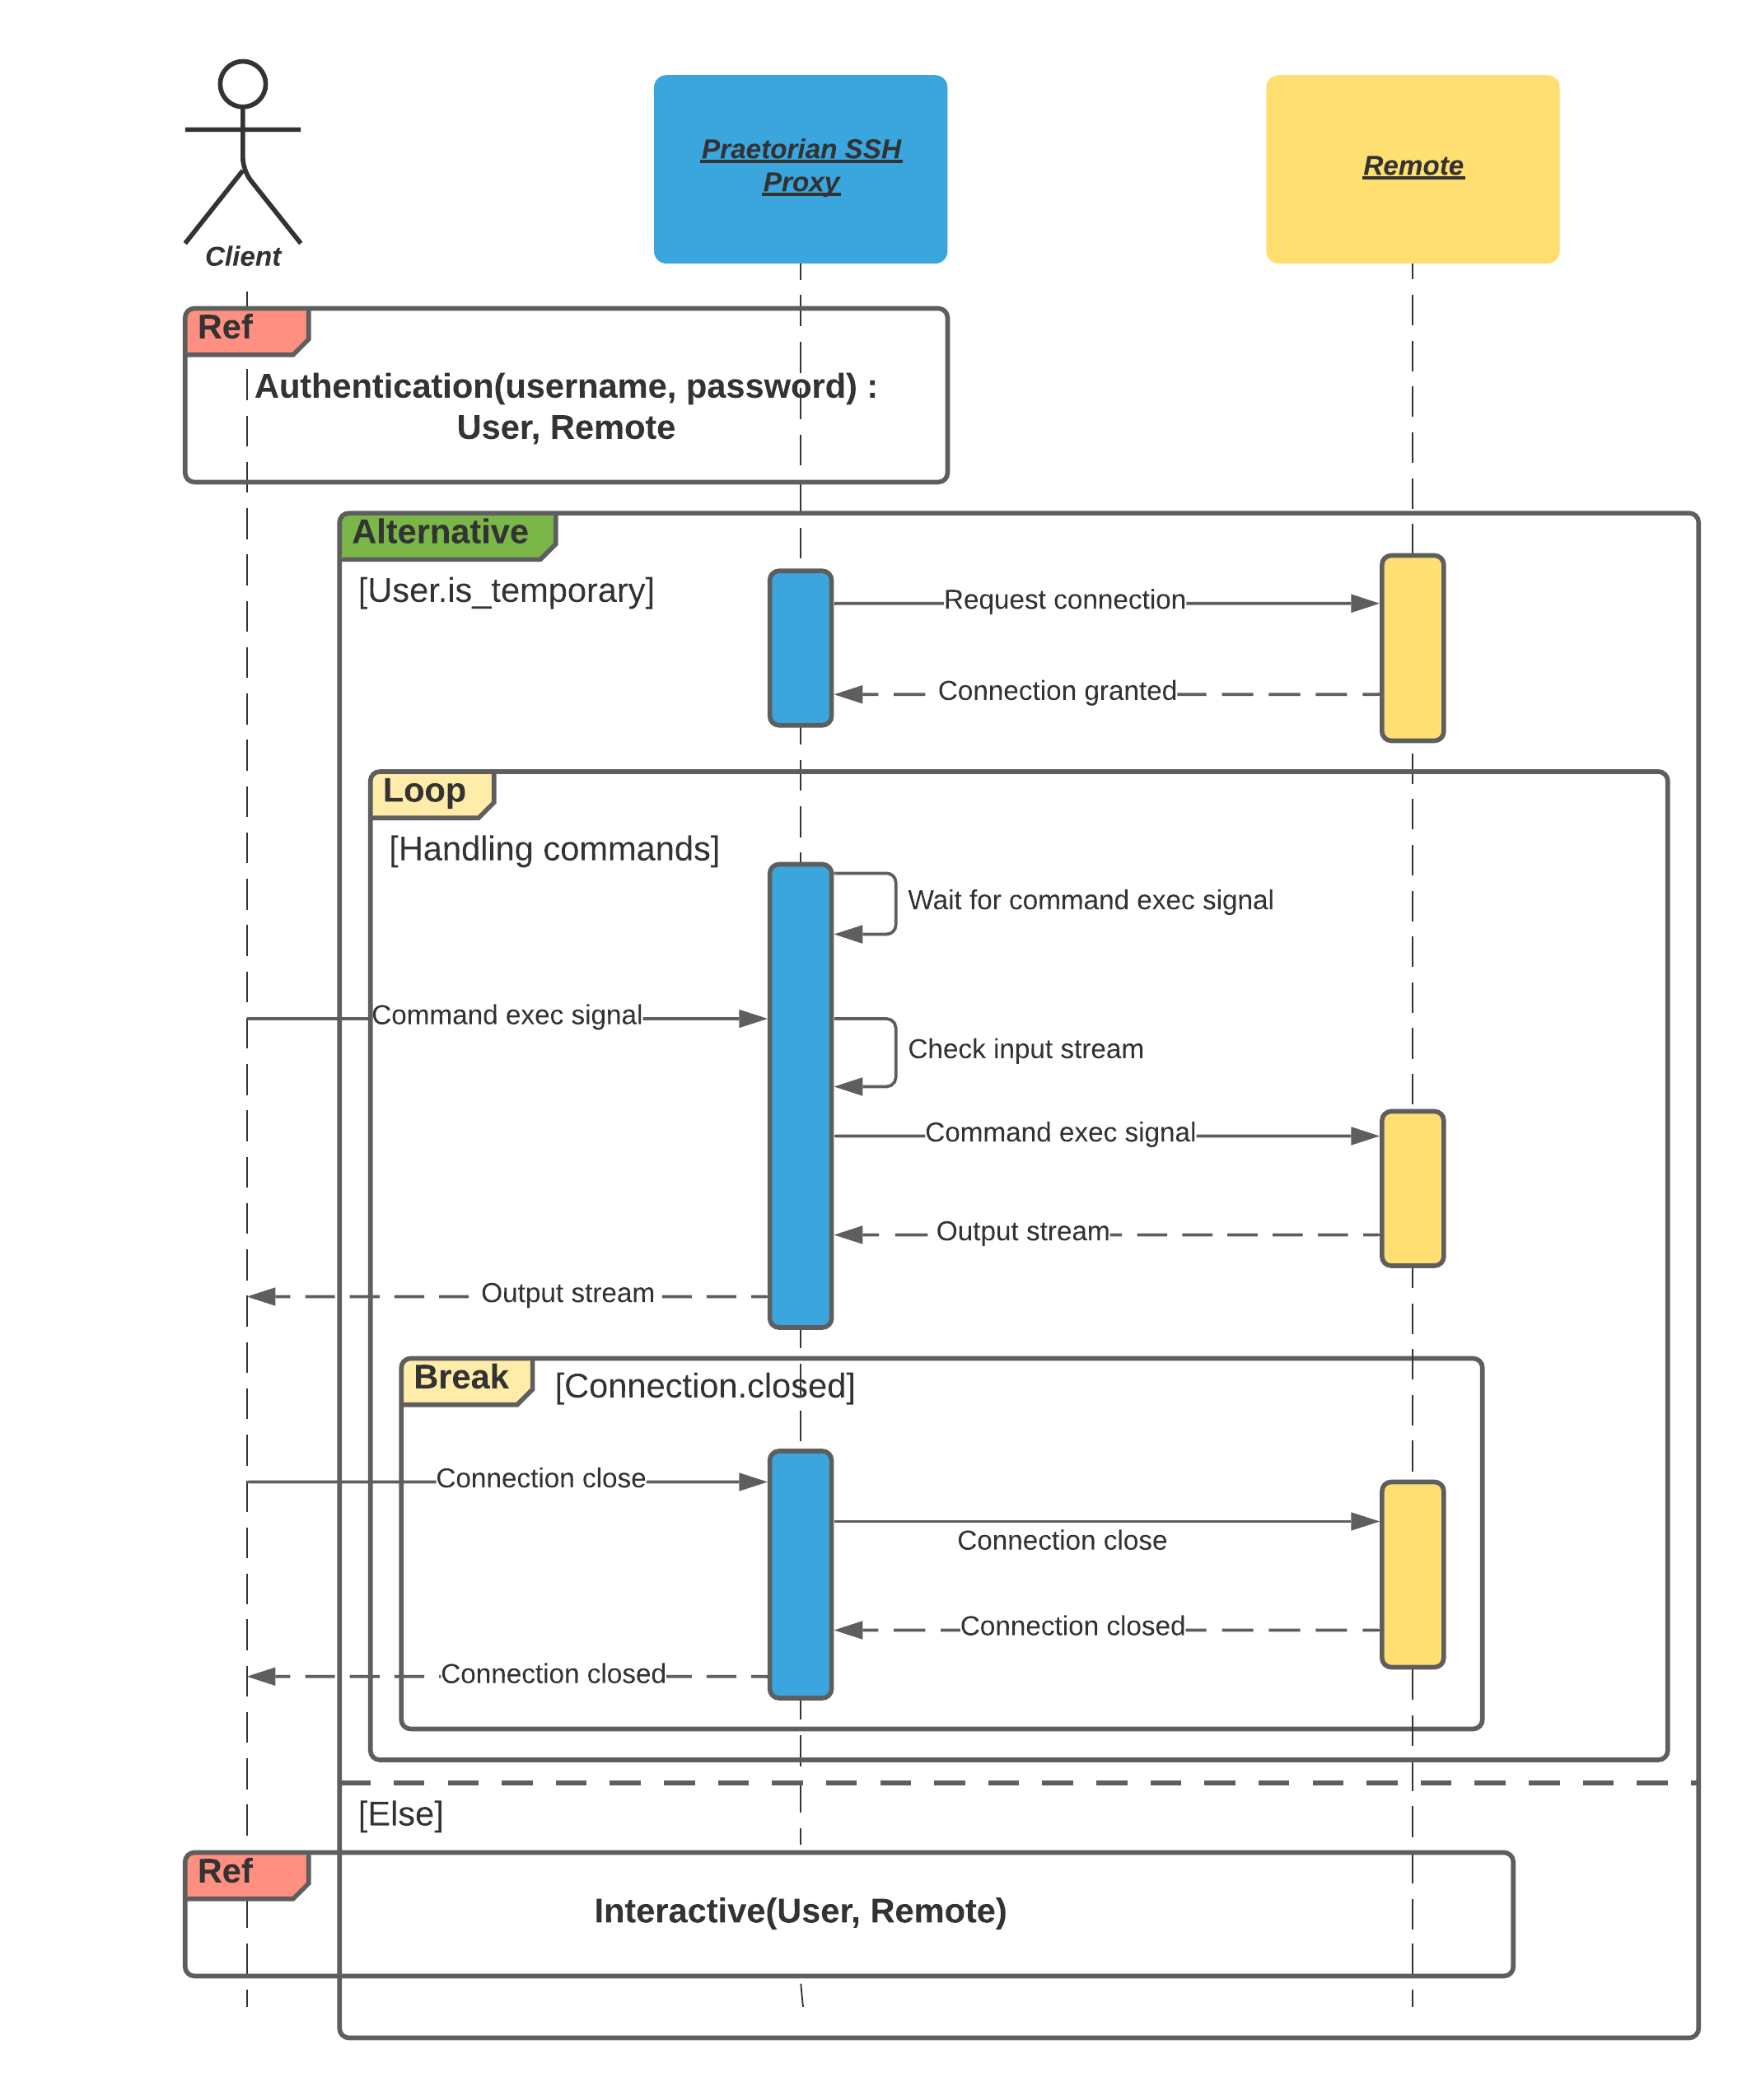
\includegraphics[width=\textwidth,height=15cm,keepaspectratio=true]{assets/sequence_diagram_non_interactive.png}\end{center}
\caption[Neinteraktívne prostredie]{Neinteraktívne prostredie}\label{fig:obr_12}
\end{figure}

Po úspešnom overení dočasného používateľa, je koncové zariadenie, na ktoré sa chce pripojiť známe, keďže dočasného používateľa
nie je možné vytvoriť na strane webovej aplikácie bez špecifikovania práve jednoho koncového zariadenia.
Tým pádom hneď po úspešnom overení totožnosti používateľa, si ssh proxy server vyžiada pripojenie na vzdialené zariadenie.
Po úspešnom pripojení k zariadeniu proxy server začne čakať na prípadné vstupy od klienta vo forme shell príkazu.
Akonáhle dostane správu, príkaz skontroluje, či neporušuje pravidlá bezpečnosti a následne ho prepošle ako príkaz do ssh
servera vzdialeného zariadenia.
Následne proxy server počká na odpoveď, ktorú po prijatí prepošle ako odpoveď klientovi.
Proxy server bude čakať a preposielať príkazy dovtedy, dokiaľ klient nepožiada o ukončenie spojenia.
Po prijatí ukončenia spojenia od klienta, proxy server pošle požiadavku o ukončenie spojenia ssh serveru koncového zariadenia
a po úspešnom uzavrení spojenia proxy server uzavrie spojenie aj s klientom.
Dané neinteraktívne rozhranie je možné použiť na veľa spôsobov, ako napríklad spracovanie skriptu, alebo súboru s príkazmi,
či pracovať so systémami, ktoré potrebujú pripojenie na ssh.
